\section{Matlab仿真与算法比较}
接下来的部分,我分别对上述算法进行了仿真,下面将分别给出相应的结果以及分析。
\subsection{ZF算法的比较}
对于ZF算法,根据其是否使用QR以及是否进行了排序,可以分为以下几类:线性ZF检测算法(Linear ZF),基于QR分解的ZF检测算法(ZF-QR SIC),基于排序和QR分解的ZF检测算法(ZF-SQRD),ZF-VBLAST检测算法(基于串行干扰消除)。\par
设定发送端和接收端天线数量均为4,使用QPSK进行调制,在瑞利衰落信道(RFC)、加性高斯白噪声(AWGN)的情况下得到在不同SNR下各算法的误比特率BER(bit error rate),并重复1000次计算平均BER,如图\ref{zf}所示。可以看出四种算法的性能差距不是非常大,其中基于串行干扰消除的ZF算法性能最好,但计算复杂度也最高。随着信噪比的不断提升,各算法的误比特率也在不断下降。\par
这也说明了在误比特率和计算复杂度、信噪比之间有一个折衷:计算复杂度高的算法准确率高,信噪比高的情况下准确率高。\par
\textit{代码和函数见文件夹zf。}
\begin{figure}[H]
\centering
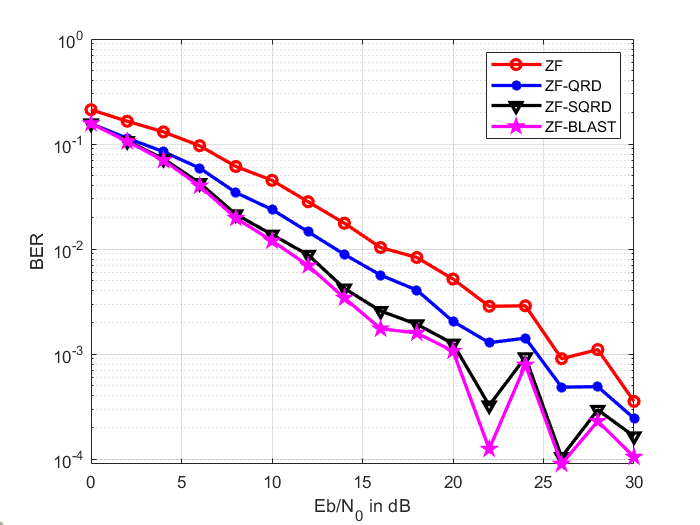
\includegraphics[scale=0.6]{zf}
\caption{不同的ZF算法仿真结果。}
\label{zf}
\end{figure}

\subsection{MMSE算法的比较}
使用与ZF算法同样的设置(天线、调制、信道、噪声、重复次数),对线性MMSE检测算法(Linear MMSE),基于QR分解的MMSE检测算法(MMSE-QR SIC),基于排序和QR分解的MMSE检测算法(MMSE-SQRD)和	MMSE-VBLAST检测算法(基于串行干扰消除)进行仿真,结果如图\ref{mmse}所示。其中MMSE-VBLAST未能成功实现,图中的曲线有误,理论上MMSE-BLAST的性能应较MMSE-SQRD更好。文章[1]中描述的ZF-BLAST算法是:将其滤波矩阵$G_{ZF}$替换为$G_{MMSE}$,并且在MMSE条件下把信道矩阵替换为扩展的信道矩阵$\underline{H}=[H;\sigma_nI_n]$作为MMSE-BLAST算法。但是失败了,网上也没有找到有效的解决方案,其原因仍待探讨。除去这点,MMSE其余三种算法的仿真性能排序与ZF相同,复杂度越高的算法准确率越高。\par
\textit{代码和函数见文件夹mmse。}
\begin{figure}[H]
\centering
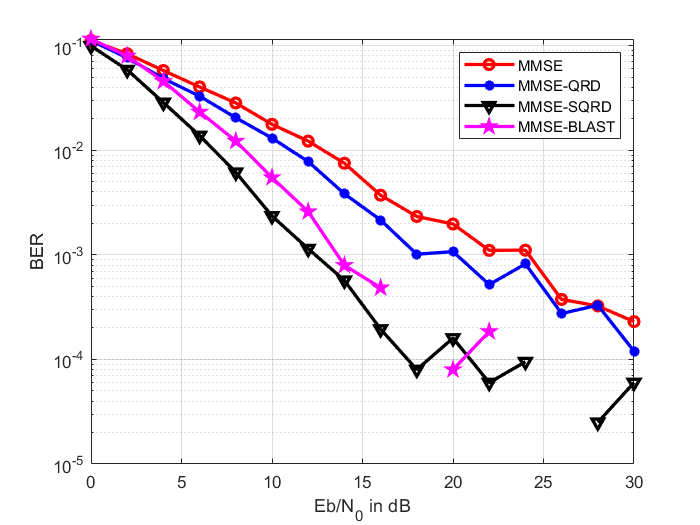
\includegraphics[scale=0.6]{mmse}
\caption{不同的MMSE算法仿真结果。}
\label{mmse}
\end{figure}

\subsection{SISO与MIMO的比较}
将信道数量设为1,此时8种算法在性能上没有区别,维持天线、调制、信道、噪声、重复次数等设置不变,任选一种算法进行仿真(这里选择了性能最好的ZF-BLAST算法),结果如图\ref{SISO}所示。\par
与图\ref{zf}和图对比知:MIMO与SISO的BER近乎相同(注意纵轴坐标),但是由于MIMO使用多天线同时发送数据,所以传输速率在不增大带宽的情况下随天线数量线性增长,并且能维持与SISO相近的正确率,充分体现了MIMO传输的优点。
\begin{figure}[H]
\centering
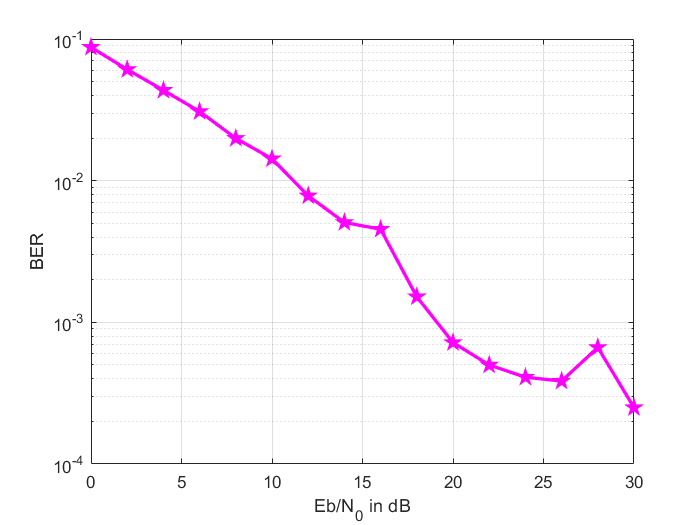
\includegraphics[scale=0.6]{SISO}
\caption{相同条件下的SISO仿真结果。}
\label{SISO}
\end{figure}

\subsection{Demo:图像传输}
将一张$100\times 100\times 3$的8位彩色图像转为二进制文件,进行QPSK调制后用4天线MIMO发送,接收端用4天线接受信号,并通过ZF-BLAST算法恢复,在三种信噪比下恢复的图像见\ref{transmit}。当SNR=10dB时,图像上有一些明显的误码(而且均为集中的突发差错);而当SNR=15dB时,图上的误码已经基本可以忽略;当SNR=20dB时,图中已经没有误码。这说明MIMO传输和ZF-BLAST恢复的性能非常好,完全能够满足图片传输的需求。\par
不过这里还有一些可以改进的地方:由于图片是直接转为二进制文件,未经过任何信源编码,所以一张$100\times 100\times 3$的8位彩色图像就需要$100\times 100\times 3\times 8=2.4\times10^5$个二进制码元来描述。一种解决方法是利用我们在project 1 中写好的JPEG 2000算法进行信源编码,压缩冗余的熵。但是由于我们组的JPEG 2000是用Python写的,而VBLAST是用Matlab写的,两者接口无法对接,在询问周小林老师后,老师说可以直接传输一张图片的二进制文件。理论上,两者连接之后传输效率能够得到很大的提升。

\textit{代码见文件夹zf中的脚本vbalst\_zf\_picture.m。}
\begin{figure}[H]
\centering
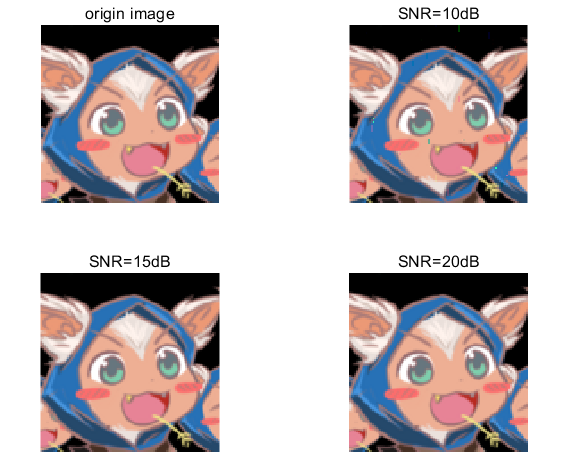
\includegraphics[scale=0.7]{transmit}
\caption{Demo:图像传输。}
\label{transmit}
\end{figure}